\documentclass[12pt]{article}

\usepackage{answers}
\usepackage{setspace}
\usepackage{graphicx}
\usepackage{enumitem}
\usepackage{multicol}
\usepackage{mathrsfs}
\usepackage[margin=1in]{geometry} 
\usepackage{amsmath,amsthm,amssymb}
\usepackage{pgfplots}
\usepackage{listings}
\pgfplotsset{compat=1.15}
\usepgfplotslibrary{fillbetween}
 
\newcommand{\N}{\mathbb{N}}
\newcommand{\Z}{\mathbb{Z}}
\newcommand{\C}{\mathbb{C}}
\newcommand{\R}{\mathbb{R}}

\DeclareMathOperator{\sech}{sech}
\DeclareMathOperator{\csch}{csch}
 
\newenvironment{theorem}[2][Theorem]{\begin{trivlist}
\item[\hskip \labelsep {\bfseries #1}\hskip \labelsep {\bfseries #2.}]}{\end{trivlist}}
\newenvironment{definition}[2][Definition]{\begin{trivlist}
\item[\hskip \labelsep {\bfseries #1}\hskip \labelsep {\bfseries #2.}]}{\end{trivlist}}
\newenvironment{proposition}[2][Proposition]{\begin{trivlist}
\item[\hskip \labelsep {\bfseries #1}\hskip \labelsep {\bfseries #2.}]}{\end{trivlist}}
\newenvironment{lemma}[2][Lemma]{\begin{trivlist}
\item[\hskip \labelsep {\bfseries #1}\hskip \labelsep {\bfseries #2.}]}{\end{trivlist}}
\newenvironment{exercise}[2][Exercise]{\begin{trivlist}
\item[\hskip \labelsep {\bfseries #1}\hskip \labelsep {\bfseries #2.}]}{\end{trivlist}}
\newenvironment{solution}[2][Solution]{\begin{trivlist}
\item[\hskip \labelsep {\bfseries #1}]}{\end{trivlist}}
\newenvironment{problem}[2][Problem]{\begin{trivlist}
\item[\hskip \labelsep {\bfseries #1}\hskip \labelsep {\bfseries #2.}]}{\end{trivlist}}
\newenvironment{question}[2][Question]{\begin{trivlist}
\item[\hskip \labelsep {\bfseries #1}\hskip \labelsep {\bfseries #2.}]}{\end{trivlist}}
\newenvironment{corollary}[2][Corollary]{\begin{trivlist}
\item[\hskip \labelsep {\bfseries #1}\hskip \labelsep {\bfseries #2.}]}{\end{trivlist}}
 
\begin{document}
 
% --------------------------------------------------------------
%                         Start here
% --------------------------------------------------------------
 
\title{Problem Set 2}%replace with the appropriate homework number
\author{Basil R. Yap\\ %replace with your name
50.021 Artificial Intelligence - Term 8} %if necessary, replace with your course title
\date{May 27, 2018}
\maketitle
%Below is an example of the problem environment

\section{Theory Component}
% Question 1
\begin{figure}[h!]
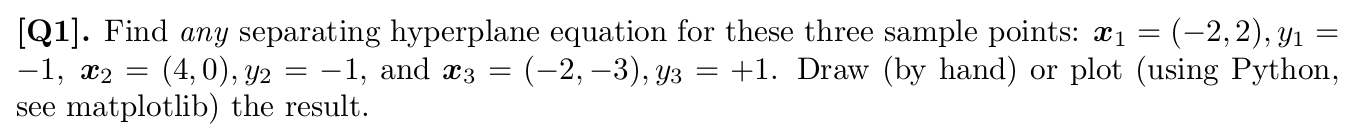
\includegraphics[width=\linewidth]{./assets/201805292051.png}
\end{figure}

\begin{solution}{}~
$$\begin{array}{ll} 
x_1=(-2,2) & y_1=-1\\
x_2=(4,0) & y_2=-1\\
x_3=(-2,-3) & y_3=+1
\end{array}$$
~\\
$$X=\left(\begin{array}{ccc}
         -2 & 2 & 1\\
         4 & 0 & 1\\
         -2 & -3 & 1
         \end{array}\right),\ \ \ \ 
Y=\left(\begin{array}{c}
         -1\\
         -1\\
         +1
         \end{array}\right)$$

$$\omega=(\omega_1,\omega_2,b)\in\mathbb R^{d+1}\\$$
$$
z=\omega x \left\{\begin{array}{ll}>0 & \text{If }y=+1\\<0 &\text{If }y=-1\\=0 &\text{If }y=0\end{array}\right.
$$

\begin{align*}
-2\omega_1+2\omega_2+b&<0\\
4\omega_1+b&<0\\
-2\omega_1-3\omega_2+b&>0\\
\end{align*}
$$\text{Any $\omega$ that satisfies this system of equations is a separating hyperplane.}$$
$$\text{Try solving for }b=0 $$
\begin{align*}
-2\omega_1+2\omega_2&<0\\
\omega_2&<\omega_1\text{ --- (1)}\\
4\omega_1&<0\\
\omega_1&<0\text{ --- (2)}\\
-2\omega_1-3\omega_2&>0\\
\omega_2&<-\frac{2}{3}\omega_1\text{ --- (3)}
\end{align*}
\begin{center}
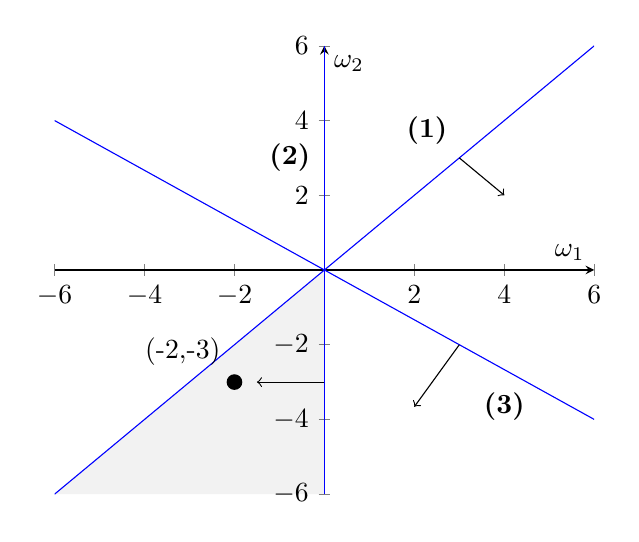
\begin{tikzpicture}
\begin{axis}[
    axis lines = left,
    axis lines = middle,
    xlabel = {$\omega_1$},
    ylabel = {$\omega_2$},
    xmax = 6
]
\path [name path=axis](-6,-6)--(6,-6);
\addplot [
    domain=-6:6, 
    samples=100,
    color=blue,
    name path=a
]
{x};
\draw[blue](0,-6)--(0,6);
\addplot [
    domain=-6:6, 
    samples=100,
    color=blue,
    name path=c
]
{-2*x/3};
\addplot [
	thick,
	color=blue,
	fill=black,
	fill opacity=0.05
] 
fill between[
	of=a and axis,
	soft clip={domain=-6:0}
];
\draw[->](3,3)--(4,2);
\draw[->](0,-3)--(-1.5,-3);
\draw[->](3,-2)--(2,-3.66);
\node[label={120:\textbf{(1)}},circle,inner sep=1pt] at (axis cs:3,3) {};
\node[label={180:\textbf{(2)}},circle,inner sep=1pt] at (axis cs:0,3) {};
\node[label={270:\textbf{(3)}},circle] at (axis cs:4,-2.66) {};
\node[label={120:{(-2,-3)}},circle,fill,inner sep=2pt] at (axis cs:-2,-3) {};
\end{axis}
\end{tikzpicture}
\end{center}
$$\text{Any value of $\omega_1$ and $\omega_2$ within the grey region is a feasible solution for the system.}$$
$$\omega_1=-2, \omega_2=-3\text{ is a feasible solution.}$$
$$\text{Below is the plot of }-2x_1-3x_2=0$$
~\\
\begin{center}
\begin{tikzpicture}
\begin{axis}[
    axis lines = left,
    axis lines = middle,
    xlabel = {$x_1$},
    ylabel = {$x_2$},
    xmax = 5,
    ymin = -4,
    ymax = 4
]
\addplot [
    domain=-4:4, 
    samples=100,
    color=blue,
]
{-2*x/3};
\node[label={120:{(-2,2)}},circle,fill,inner sep=2pt] at (axis cs:-2,2) {};
\node[label={120:{(4,0)}},circle,fill,inner sep=2pt] at (axis cs:4,0) {};
\node[label={120:{(-2,-3)}},circle,draw,inner sep=2pt] at (axis cs:-2,-3) {};
\end{axis}
\end{tikzpicture}
\end{center}
\end{solution}

\pagebreak

% Question 2
\begin{figure}[h!]
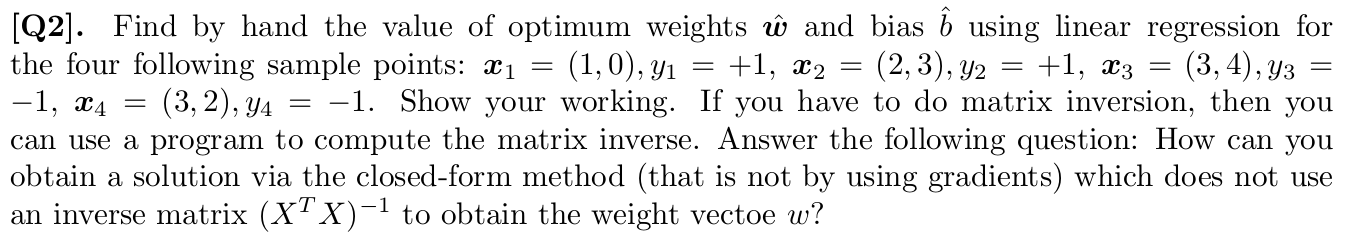
\includegraphics[width=\linewidth]{./assets/201805292053.png}
\end{figure}

\begin{solution}{}~
$$\begin{array}{ll} 
x_1=(1,0) & y_1=+1\\
x_2=(2,3) & y_2=+1\\
x_3=(3,4) & y_3=-1\\
x_4=(3,2) & y_4=-1
\end{array}$$
~\\
$$X=\left(\begin{array}{ccc}
         1 & 0 & 1\\
         2 & 3 & 1\\
         3 & 4 & 1\\
         3 & 2 & 1
         \end{array}\right),\ \ \ \ 
Y=\left(\begin{array}{c}
         +1\\
         +1\\
         -1\\
         -1
         \end{array}\right)$$

$$\omega=(\omega_1,\omega_2,b)\in\mathbb R^{d+1}\\$$
$$
z=\omega x \left\{\begin{array}{ll}>0 & \text{If }y=+1\\<0 &\text{If }y=-1\\=0 &\text{If }y=0\end{array}\right.
$$
~\\
$$\text{Using Mean Square Error as the point loss function, }\mathcal L_1=\frac{1}{2}(y-\omega x)^2$$
Through a series of operations (proven in the previous problem set and various various resources online), we arrive at the gradient function of the average loss value below\cite{proof1}:
$$\nabla\mathcal L_n(y,z(\omega;x))=\frac{1}{N}(X^TX\omega-X Y)$$
$$\text{We then find the exact solution at the turning point, }\nabla\mathcal L_n(y,z(\omega;x))=0$$
\begin{align*}
\frac{1}{N}(X^TX\ \hat\omega-X Y) &= 0\\
X^TX\ \hat\omega-X Y&= 0\\
X^TX\ \hat\omega &= X Y \\
\hat\omega &= (X^TX)^{-1}X^TY
\end{align*}
\pagebreak
$$\hat\omega=\left(\left[\begin{matrix}
1&2&3&3\\0&3&4&2\\1&1&1&1
\end{matrix}\right]\left[\begin{matrix}
1&0&1\\2&3&1\\3&4&1\\3&2&1
\end{matrix}\right]\right)^{-1}\left[\begin{matrix}
1&2&3&3\\0&3&4&2\\1&1&1&1
\end{matrix}\right]\left[\begin{matrix}
1\\1\\-1\\-1
\end{matrix}\right]$$
~\\
$$\text{Using a calculator,}$$
$$\hat\omega=\left[\begin{matrix}
-1.5\\0.3\\2.7
\end{matrix}\right]$$
$$\hat\omega=\left[\begin{matrix}
-1.5\\0.3
\end{matrix}\right]*,\ \ \ \ \hat b=2.7$$

$$*\ \hat\omega\textit{ as defined by the question.}$$
~\\
To solve for an optimal solution $\hat\omega$ with a closed-form method without use of an inverse matrix, there are three possible cases to consider. The system of equations (i.e. the number of observations with respect to the number of dimensions/variables) can be \textbf{under-determined},\textbf{solvable} or  \textbf{over-determined}.\\

When the system of equations is \textbf{under-determined}, there are not enough observations to properly define $\hat\omega$ such that there is a single unique solution to the system of equations. In this case, the system of equations can be solved loosely with respect to $\hat\omega$ and a range/set of optimal values can be found.\\

When the system of equations is \textbf{solvable}, there are perfectly sufficient observations to solve for a unique $\hat\omega$. By simply solving the system of equations via simultaneous or row echelon method, a single unique solution for $\hat\omega$ can be found.\\

When the system of equations is \textbf{over-determined}, the number of observations is more than sufficient solve for $\hat\omega$, to the point where the value of $\hat\omega$ calculated may not hold true for all observations (this occurs when the data is not linearly separable). Other than an analytical solution using an inverse matrix or gradient descent, perhaps the only other way to get a reasonable estimate of $\hat\omega$ would be to solve the system of equation using the row echelon method and then subsequently relaxing the problem by dropping rows/observations from the matrix. This would provide a reasonable solution for most observations, but may not result in the lowest possible loss value.

\end{solution}

\pagebreak

% Question 3
\begin{figure}[h!]
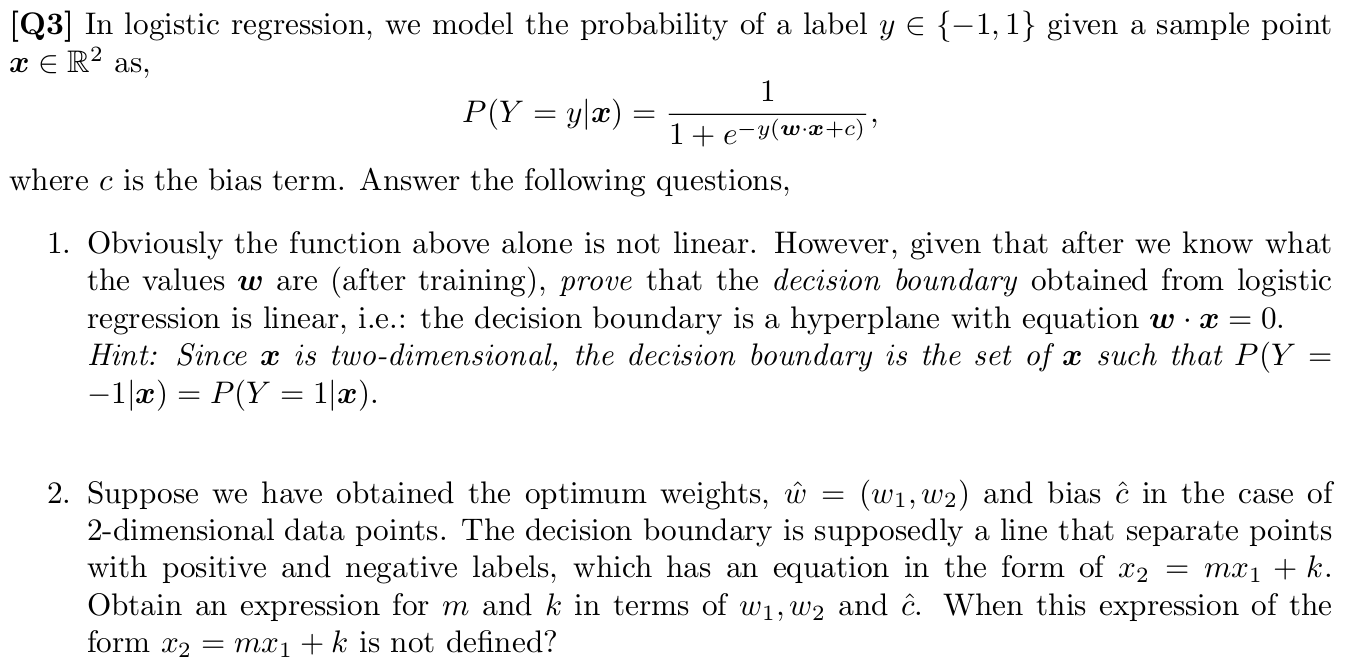
\includegraphics[width=\linewidth]{./assets/201805292055.png}
\end{figure}

\begin{solution}{}~
\begin{enumerate}[label=\arabic*)]
\item For any given $x$, the boundary condition would be when there is an equal likelihood of $Y=-1$ and $Y=+1$.\\
\begin{align*}
\therefore\text{Evaluate }\Pr(Y=-1|x)&=\Pr(Y=+1|x)\\
\frac{1}{1+e^{\omega\cdot x+c}}&=\frac{1}{1+e^{-(\omega\cdot x+c)}}\\
1+e^{\omega\cdot x+c}&=1+e^{-(\omega\cdot x+c)}\\
e^{\omega\cdot x+c}&=e^{-(\omega\cdot x+c)}\\
\omega\cdot x+c&=-(\omega\cdot x+c)\\
\omega\cdot x+c&=0
\end{align*}
$$\therefore\text{The decision boundary is linear.}$$
\item From \textbf{Part 1}, the decision boundary line can be defined by $\omega\cdot x+c=0$\\

$$\text{Now consider for the case when weights and bias are optimal, }\hat\omega\cdot x+\hat c=0$$
$$
\left[\begin{matrix}
\omega_1 & \omega_2
\end{matrix}\right]\cdot\left[\begin{matrix}
x_1 \\ x_2
\end{matrix}\right]+\hat c=0
$$
\begin{align*}
\omega_1 x_1+\omega_2 x_2+\hat c&=0\\
\omega_2 x_2&=-\omega_1 x_1-\hat c\\
x_2&=-\frac{\omega_1}{\omega_2}x_1-\frac{\hat c}{\omega_2}\\
m=-\frac{\omega_1}{\omega_2}\ ,&\ k=-\frac{\hat c}{\omega_2}
\end{align*}
$$x_2=mx_1+k\text{ is not defined when }\omega_2=0$$
\end{enumerate}
\end{solution}

% Question 4
\begin{figure}[h!]
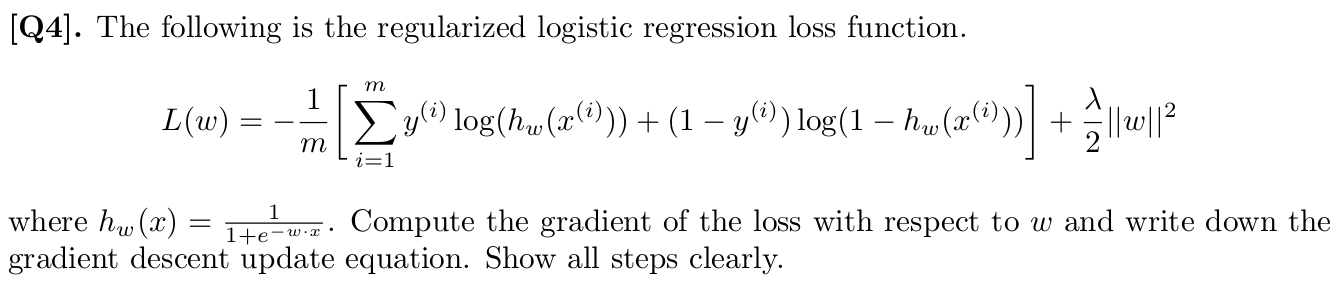
\includegraphics[width=\linewidth]{./assets/201805292056.png}
\end{figure}

\begin{solution}{}~
$$\mathcal L(\omega)=-\frac{1}{m}\left[\sum_{i=1}^my^{(i)}\log(h_\omega(x^{(i)}))+(1-y^{(i)})\log(1-h_\omega(x^{(i)}))\right]+\frac{\lambda}{2}||\omega||^2\\$$
\begin{align*}
\nabla\mathcal L(\omega)&=\frac{d}{d\omega}\left(-\frac{1}{m}\left[\sum_{i=1}^my^{(i)}\log(h_\omega(x^{(i)}))+(1-y^{(i)})\log(1-h_\omega(x^{(i)}))\right]+\frac{\lambda}{2}||\omega||^2\right)\\
&=-\frac{1}{m}\left[\sum_{i=1}^my^{(i)}\frac{h_\omega'(x^{(i)})}{h_\omega(x^{(i)})}+(1-y^{(i)})\frac{-h_\omega'(x^{(i)})}{1-h_\omega(x^{(i)})}\right]+\lambda\omega
\end{align*}
$$h_\omega(x)=\frac{1}{1+e^{-\omega\cdot x}}$$
\begin{align*}
h_\omega'(x)&=\frac{d}{d\omega}\left(\frac{1}{1+e^{-\omega\cdot x}}\right)\\
&=-\left(\frac{1}{(1+e^{-\omega\cdot x})^2}\right)(-xe^{-\omega\cdot x})\\
&=xh_\omega(x)^2e^{-\omega\cdot x}
\end{align*}
\begin{align*}
\nabla\mathcal L(\omega)&=-\frac{1}{m}\left[\sum_{i=1}^my^{(i)}\frac{x^{(i)}h_\omega(x^{(i)})^2e^{-\omega\cdot x^{(i)}}}{h_\omega(x^{(i)})}+(1-y^{(i)})\frac{-x^{(i)}h_\omega(x^{(i)})^2e^{-\omega\cdot x^{(i)}}}{1-h_\omega(x^{(i)})}\right]+\lambda\omega\\
&=-\frac{1}{m}\left[\sum_{i=1}^my^{(i)}x^{(i)}e^{-\omega\cdot x^{(i)}}h_\omega(x^{(i)})+(y^{(i)}-1)(x^{(i)}e^{-\omega\cdot x^{(i)}})\frac{h_\omega(x^{(i)})^2}{1-h_\omega(x^{(i)})}\right]+\lambda\omega
\end{align*}
\pagebreak
$$\text{For each }k\text{ step size, the new loss function value is given by}$$
$$\mathcal L(\omega')\leftarrow \mathcal L(\omega)+k\nabla\mathcal L(\omega)$$
\begin{align*}
\mathcal L(\omega)+k\nabla\mathcal L(\omega)&=-\frac{1}{m}\left[\sum_{i=1}^my^{(i)}\log(h_\omega(x^{(i)}))+(1-y^{(i)})\log(1-h_\omega(x^{(i)}))\right]+\frac{\lambda}{2}||\omega||^2\\
&-\frac{1}{m}\left[\sum_{i=1}^my^{(i)}x^{(i)}e^{-\omega\cdot x^{(i)}}h_\omega(x^{(i)})+(y^{(i)}-1)(x^{(i)}e^{-\omega\cdot x^{(i)}})\frac{h_\omega(x^{(i)})^2}{1-h_\omega(x^{(i)})}\right]+\lambda\omega
\end{align*}
\end{solution}

\section{Coding Component}

\lstinputlisting[language=Python]{pset2.py}

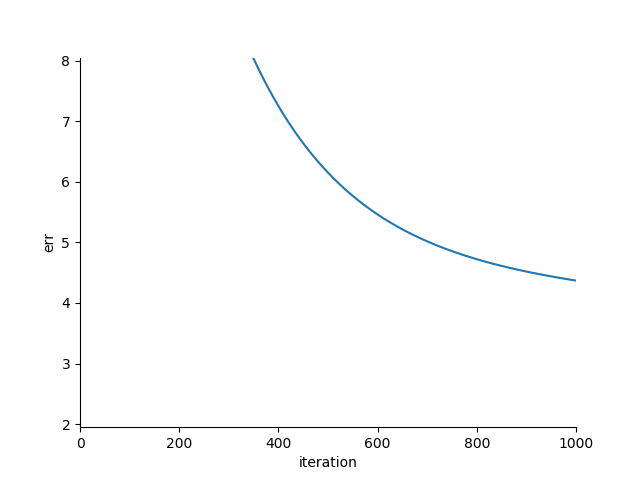
\includegraphics[width=\linewidth]{./assets/201805301419.png}
\pagebreak
\begin{figure}[h!]
\centering
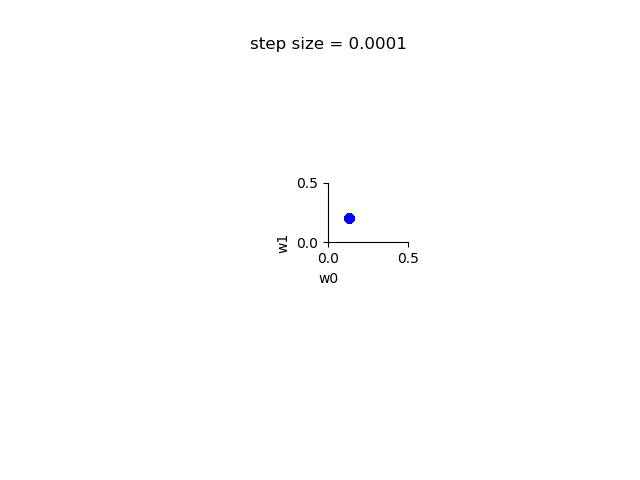
\includegraphics[width=.45\linewidth]{./assets/201805301420.png}
\centering
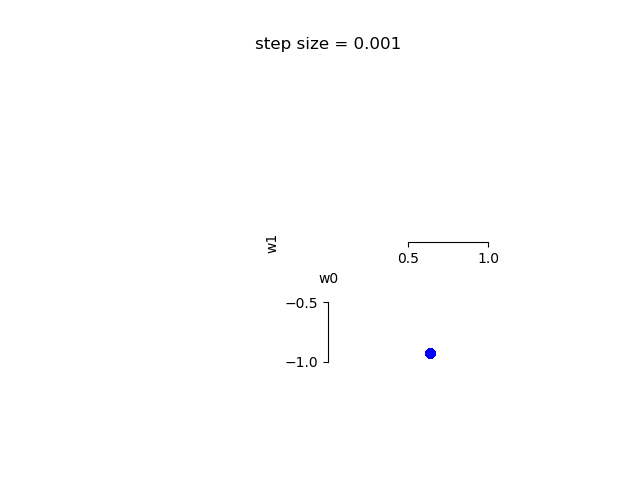
\includegraphics[width=.45\linewidth]{./assets/201805301421.png}
\end{figure}
\begin{figure}[h!]
\centering
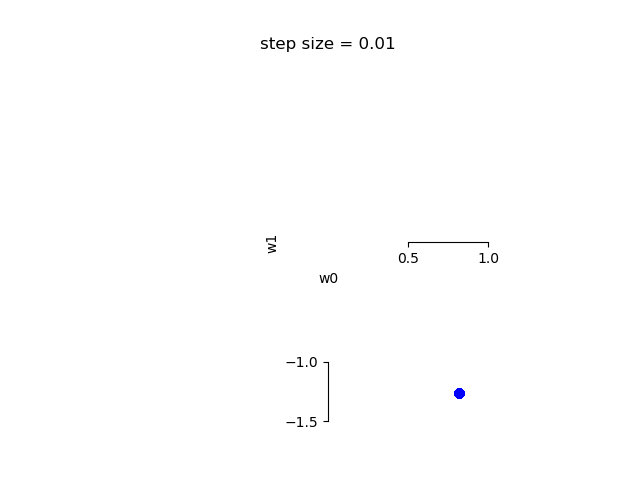
\includegraphics[width=.45\linewidth]{./assets/201805301422.png}
\centering
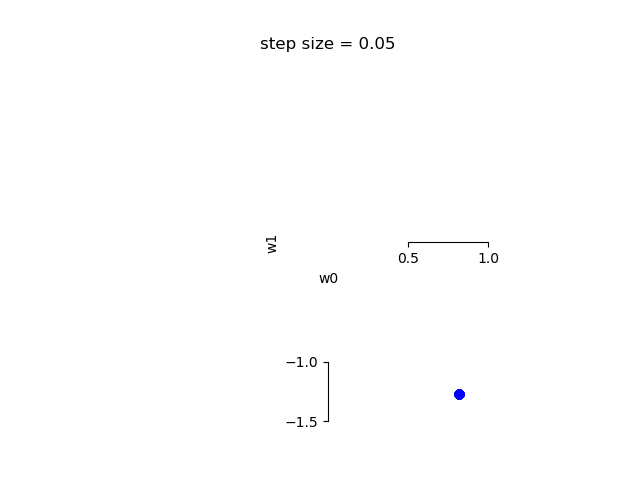
\includegraphics[width=.45\linewidth]{./assets/201805301423.png}
\end{figure}
\begin{figure}[h!]
\centering
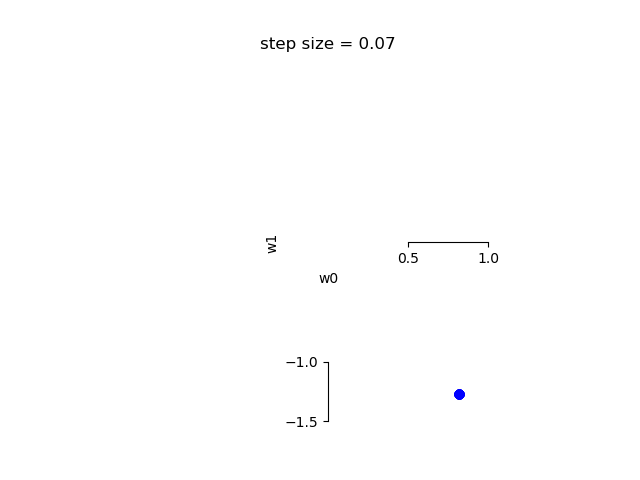
\includegraphics[width=.45\linewidth]{./assets/201805301424.png}
\centering
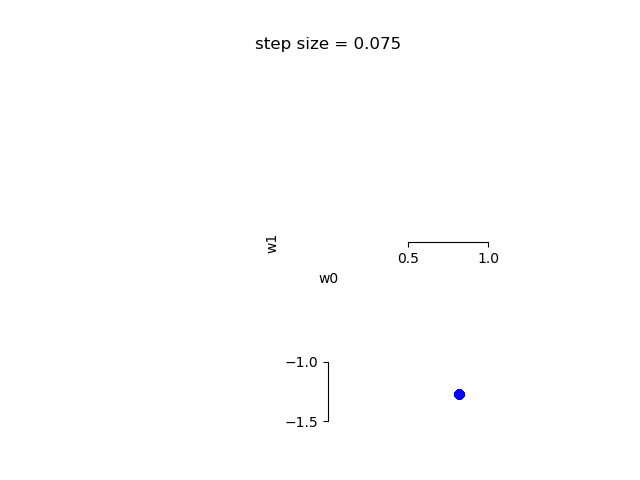
\includegraphics[width=.45\linewidth]{./assets/201805301425.png}
\end{figure}
\pagebreak
\begin{figure}[h!]
\centering
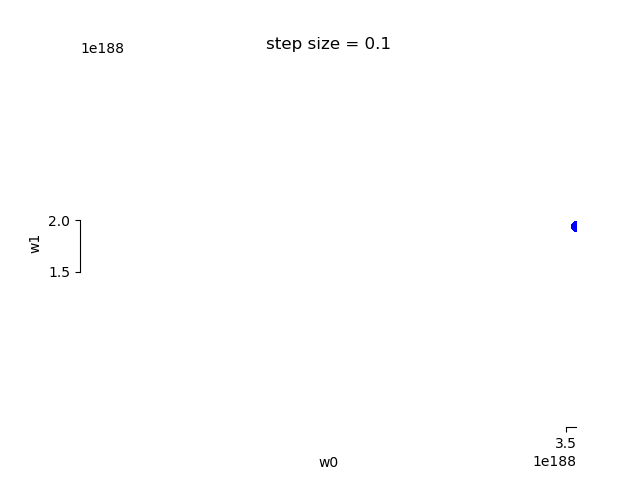
\includegraphics[width=.45\linewidth]{./assets/201805301426.png}
\end{figure}

\begin{thebibliography}{9}
\bibitem{proof1} Ng, A. (2000). CS229 Lecture notes. \emph{CS229 Lecture notes}, \emph{1}(1), 11.
\end{thebibliography}

\end{document}
